\documentclass{beamer}
<<<<<<< HEAD
\usepackage{beamerthemesplit} 
=======
%\usepackage{beamerthemesplit}
>>>>>>> 74eaa76cfe943b47547e1819b9b37f649b49f6ce
\title{Computational Physics Group Project: \\ Ecosystem: predator and prey}
\author{David Hicks\\ Weiyao Ke \\ Shagun Maheshwari \\ Fan Zhang}
\date{\today}

\begin{document}
`	
\frame{\titlepage}

\section[Outline]{}
\frame{\tableofcontents}

\section{Introduction to eco-system modelling}
\frame
{
  \frametitle{Population interaction of predator and prey in eco-system}
  %Add what you want here
\begin{figure}[htbp]
\begin{center}
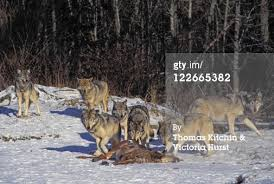
\includegraphics[width=0.9\textwidth]{predator_prey.jpg}
\caption{default}
\label{default}
\end{center}
\end{figure}

  
}
\frame
{
  \frametitle{A simplified determinsitic model L-V equation}
  %Add what you want here
  
}
\frame
{
  \frametitle{Simulation of a eco-system with predator and prey}
  %Add what you want here
  
}

\section{Implementation of the simulation}
\frame
{
  \frametitle{Structural setup}
  %Add what you want here
  
}

\frame
{
  \frametitle{Initialization}
  %Add what you want here
  
}

\frame
{
  \frametitle{time evolution}
  %Add what you want here
  
}

\frame
{
  \frametitle{parameter scanning}
  %Add what you want here
\begin{figure}[htbp]
\begin{center}
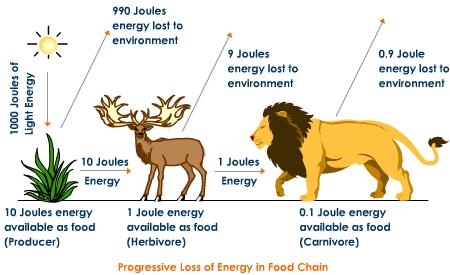
\includegraphics[width=0.9\textwidth]{progressive-energy-loss.jpeg}
\caption{default}
\label{default}
\end{center}
\end{figure}

  
}

\frame
{
  \frametitle{Parameter Search}
  \underline{5 parameters to test (5-D parameter space)}
  \begin{itemize}
  \item{\textbf{Initial population of deer}}
  \item{\textbf{Initial population of wolves}}
  \item{Reproduction age of deer}
  \item{Reproduction age of wolf}
  \item{Starvation "age" of wolf}
  \end{itemize} 

  \underline{Reduce to 4 dimensions (4-D)}
  \begin{itemize}
  \item{\textbf{Ratio of initial populations : Size of point}}
  \item{Reproduction age of deer : x-axis}
  \item{Reproduction age of wolf : y-axis}
  \item{Starvation "age" of wolf : z-axis}
  \end{itemize} 

}
\frame
{
  \frametitle{Results of Full Parameter Search}
}

\frame
{
  \frametitle{Results of Restricted Parameter Search}
  \center{Fix initial population ratios}
  \begin{figure}[H]
  \centering
        \begin{tabular}{@{}cc@{}cc@{}}
                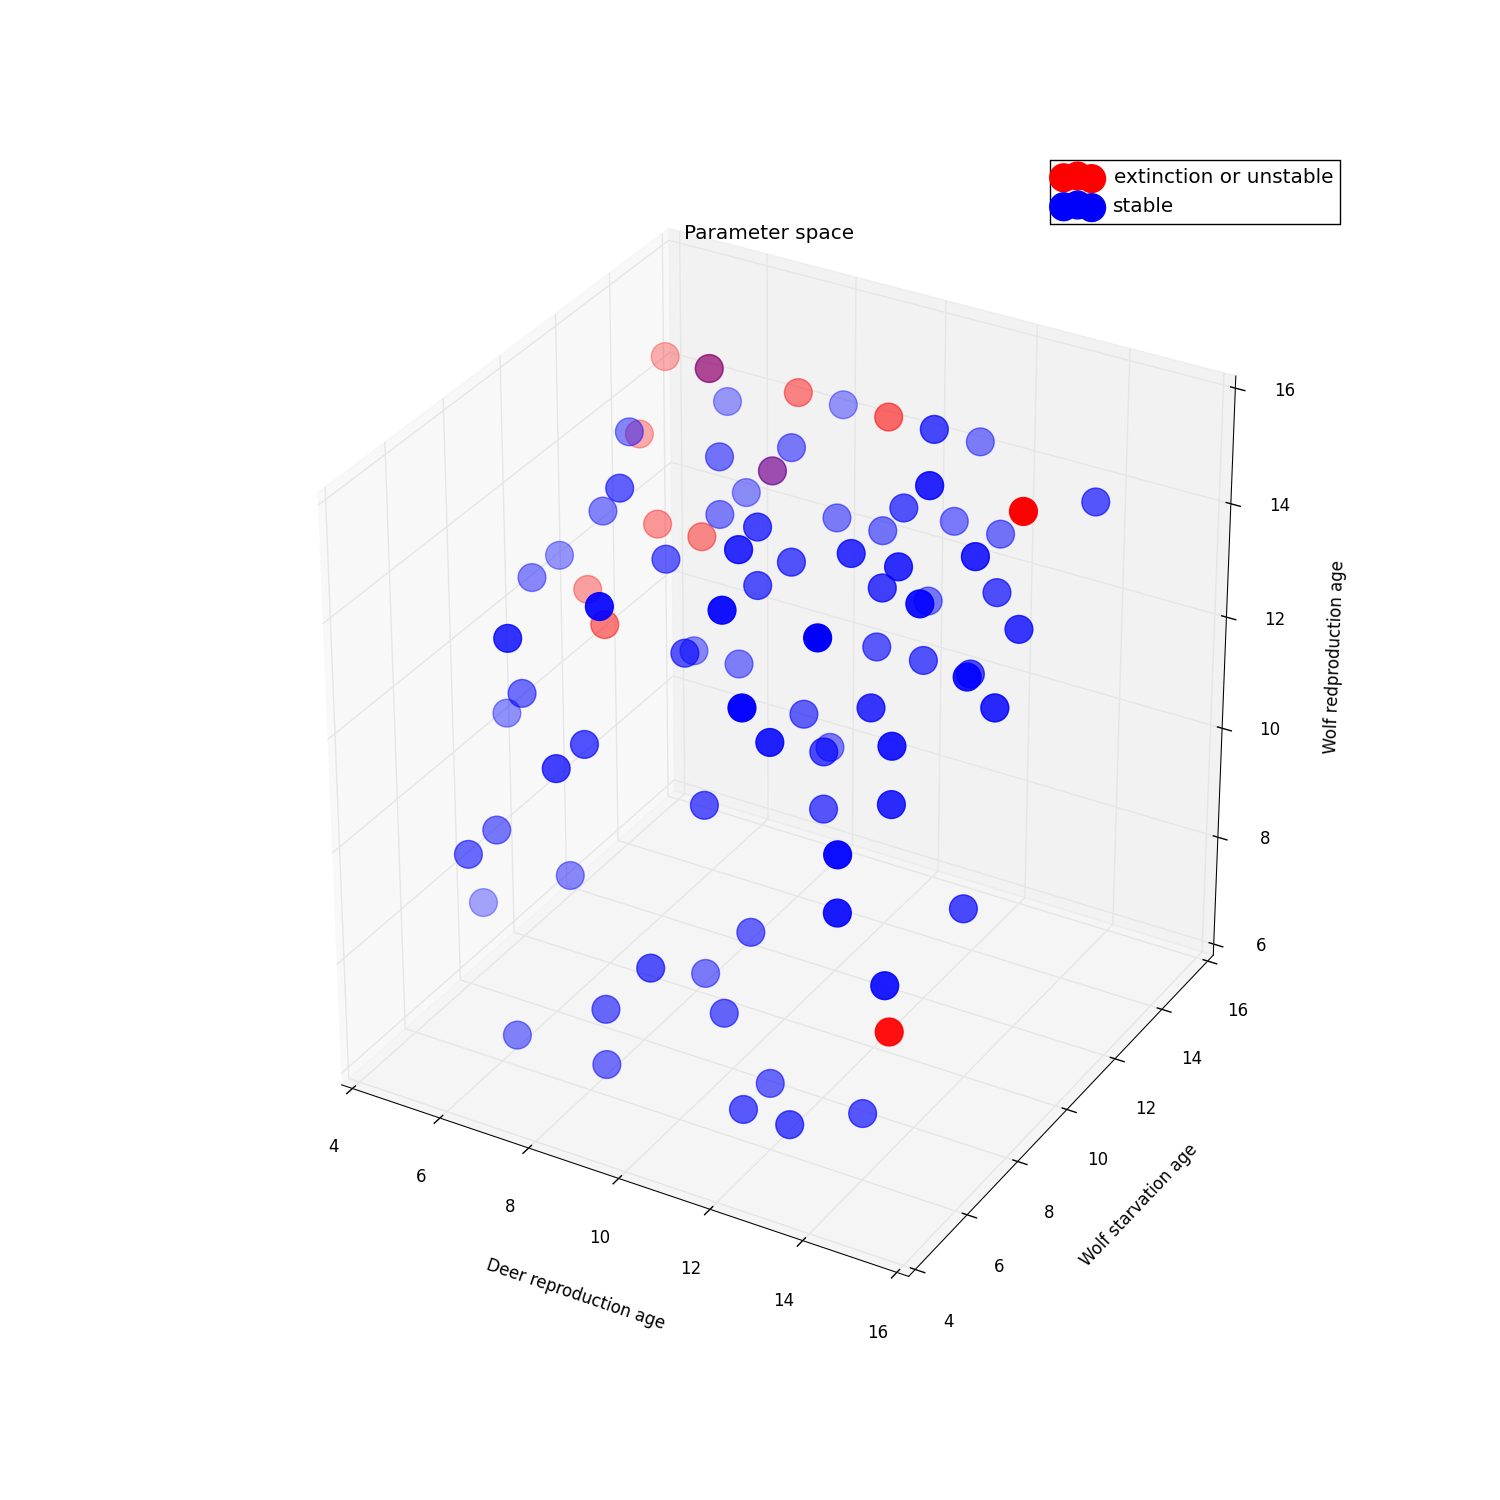
\includegraphics[width = 0.3\textwidth]{Restricted_Parameter_space_d2500_w250.png} &
                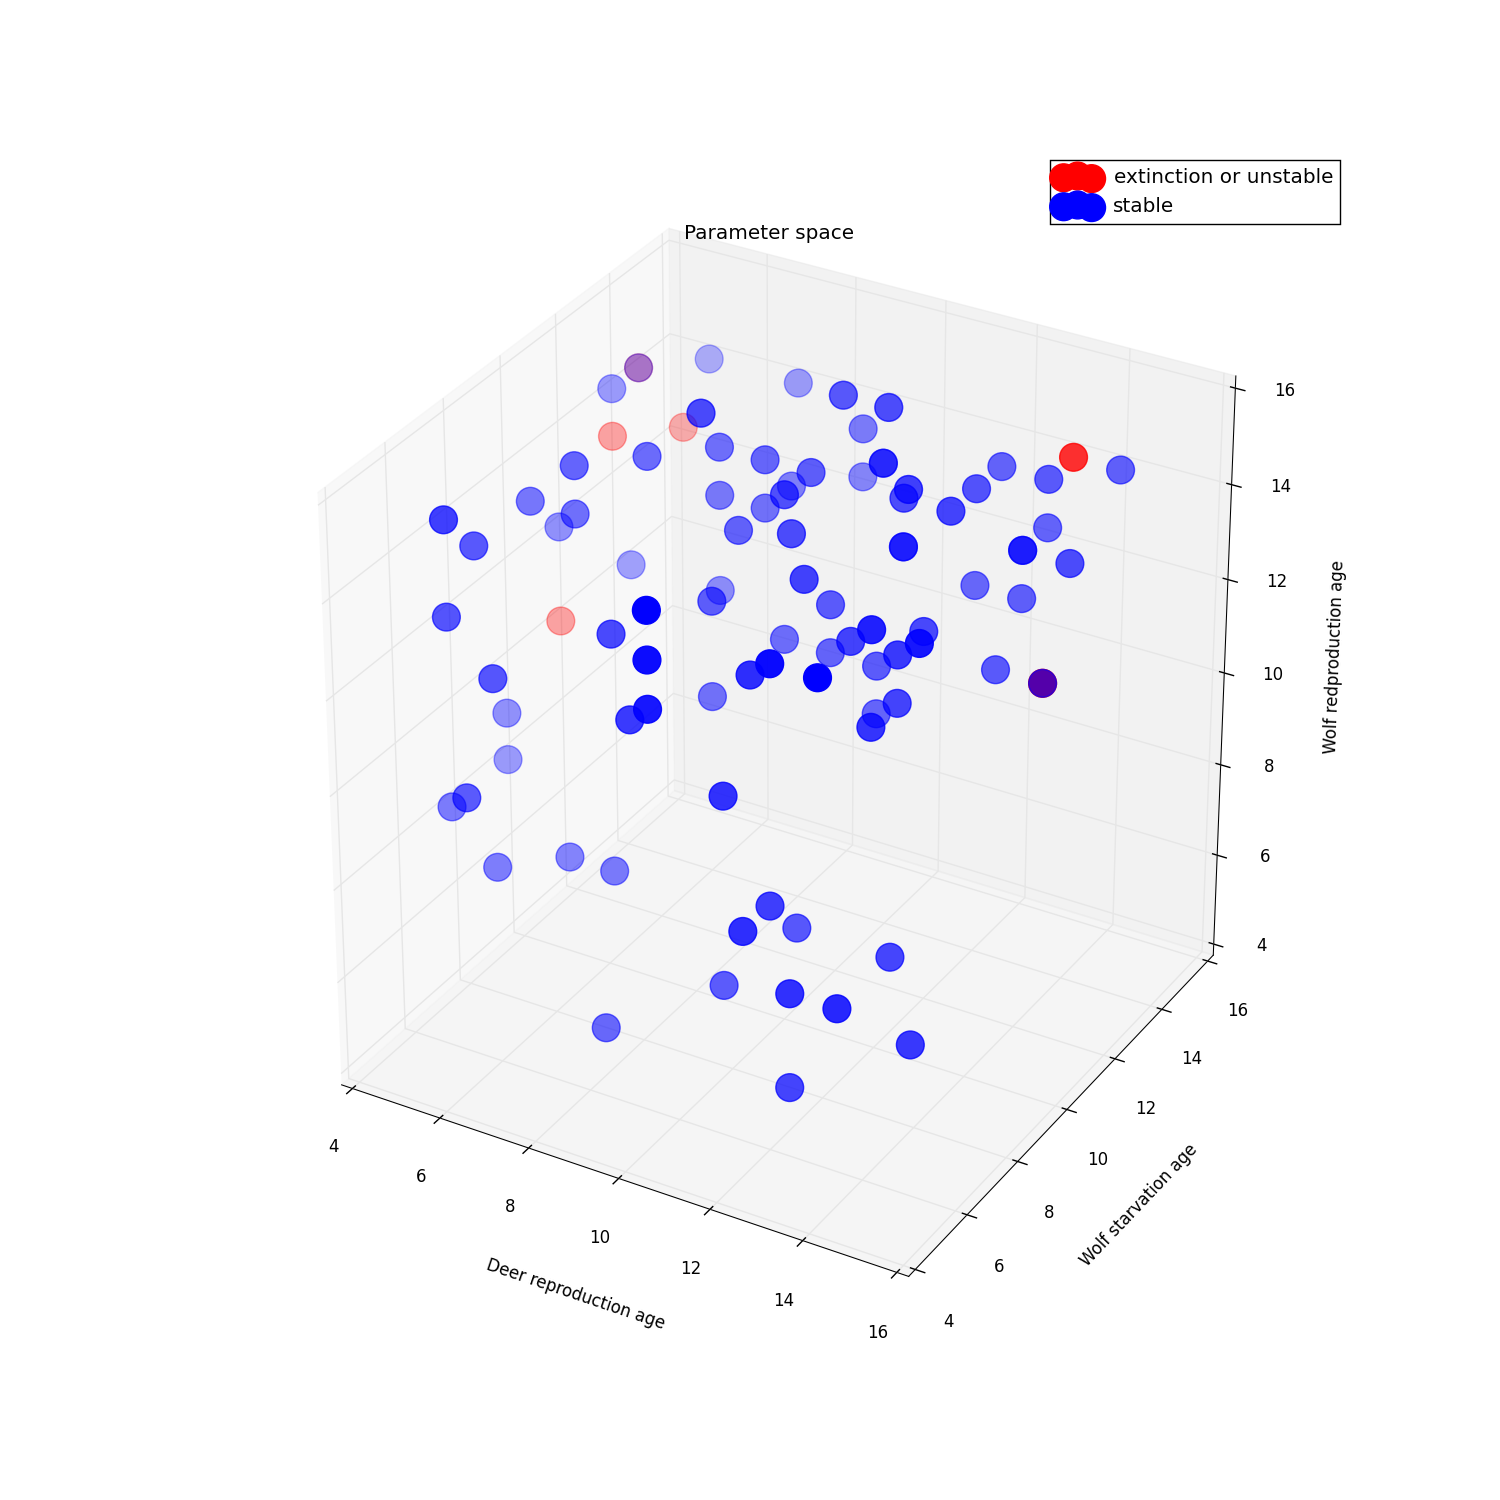
\includegraphics[width = 0.3\textwidth]{Restricted_Parameter_space_d3000_w500.png} &
                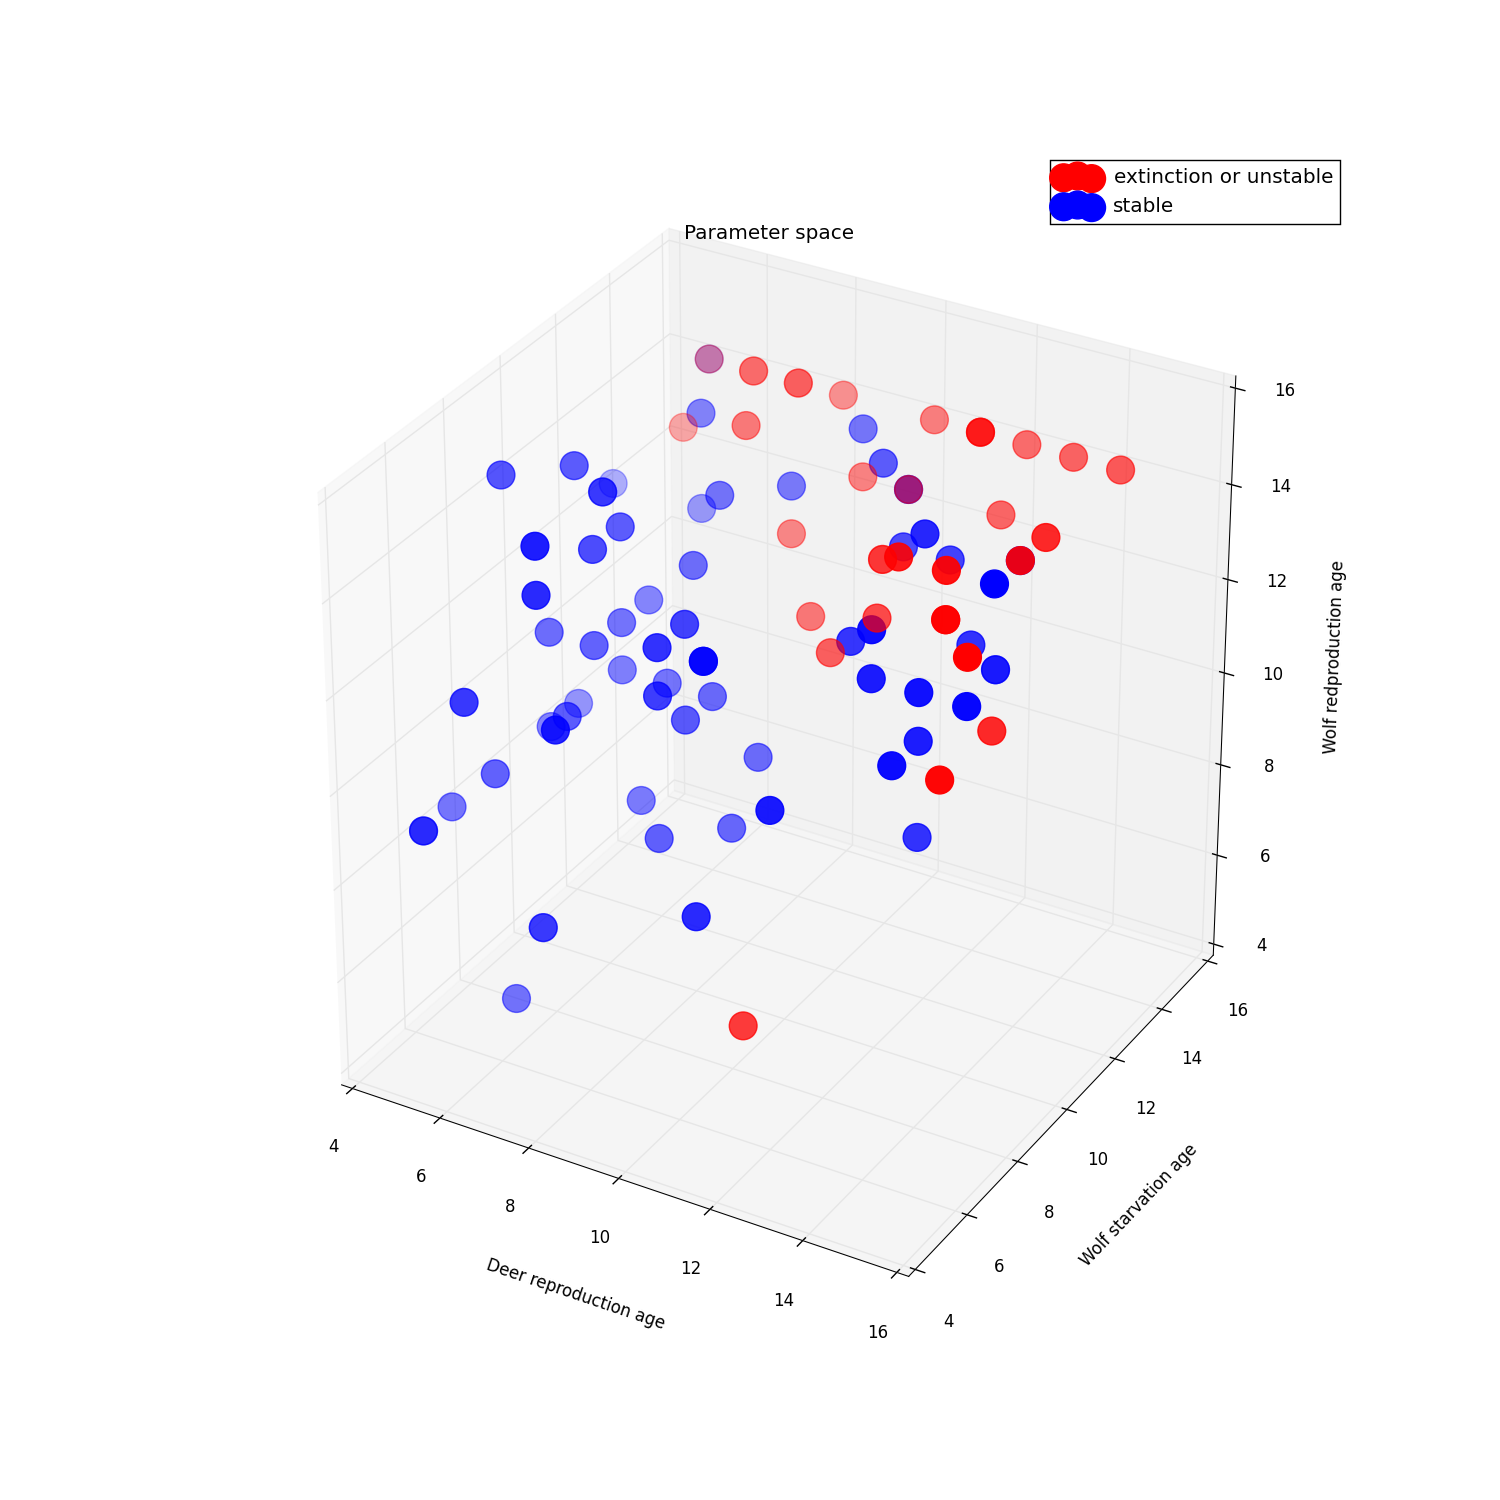
\includegraphics[width = 0.3\textwidth]{Restricted_Parameter_space_d2000_w2000.png} \\
                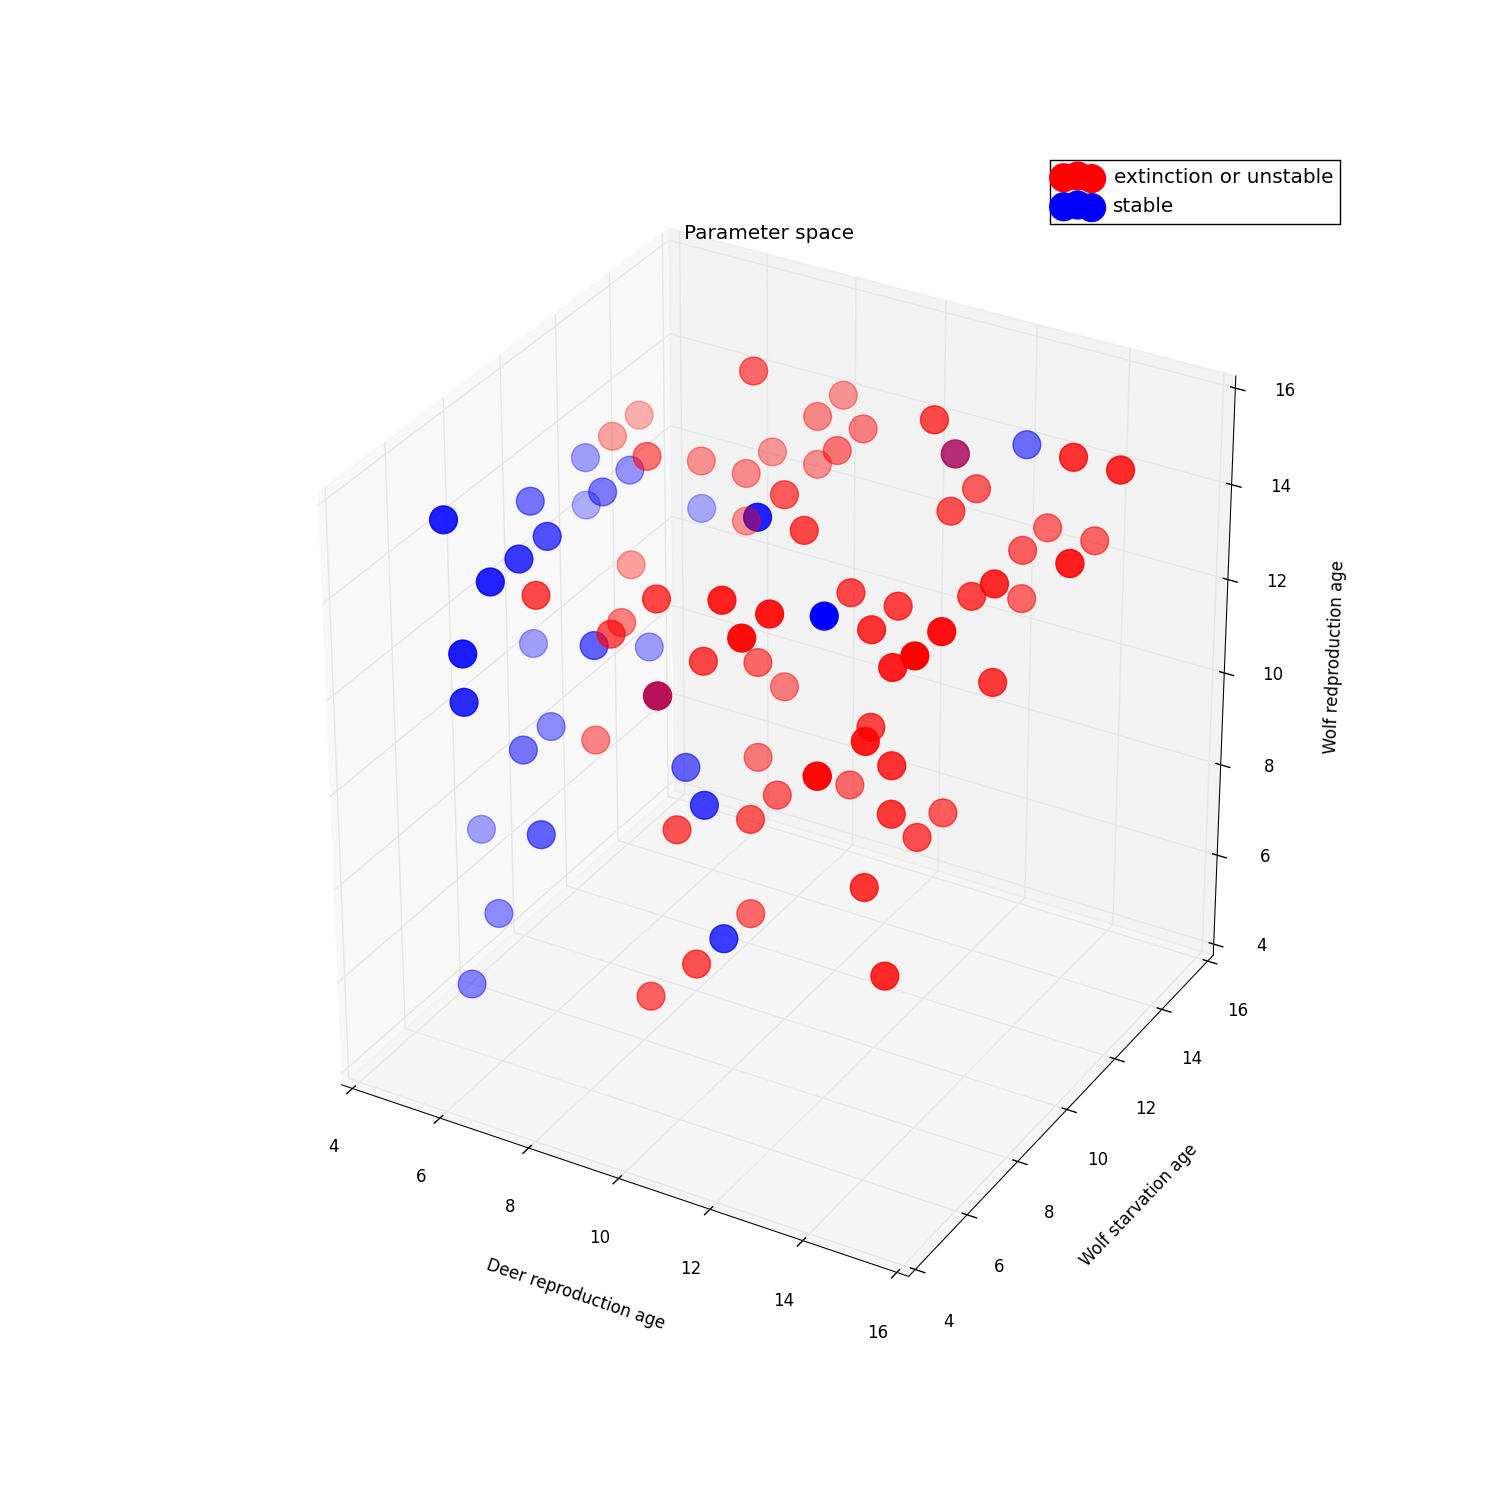
\includegraphics[width = 0.3\textwidth]{Restricted_Parameter_space_d500_w3000.png} \\
        \end{tabular}
        \label{RestrictParam}
  \end{figure}


}



\section{Results and discussion}
\frame
{
  \frametitle{Ecosystem at Equilibrium}
  Parameters used:  .........



  %Add what you want here
  
}


\end{document}
